\chapter{Systems Level Design}
\graphicspath{{images/}}
%--------------------------------------------------------------------------------
%
%--------------------------------------------------------------------------------
\section{Customer Needs and Requirements Flowdown}
% refer to PDS, market survey report, QFD, as needed
Even after wildland fires have been contained, they present many potentially hazardous environments for people. Residual smoke can make large areas of land unsafe for human traffic, especially for prolonged periods of time. Fire fighters, however, have to continue to work in these areas after the initial fire is contained, exposing themselves to unsafe levels of contamination. This creates a need for an unmanned vehicle that can be deployed in backcountry areas. 

%interviews, from customer needs report
In order to better understand the needs of the current market, our team interviewed some potential users. Three persons were interviewed: Antoinne "Chidi" Untamed, a Forest Firefighter at ASI Arden Solutions Inc., Max Reese, a Volunteer Search and Rescue First Responder, and Matthew Perez, Lieutenant Firefighter, Santa Clara Fire Department. 

When interviewed, interest was expressed right away for a product that could provide ground level environmental sensing to firefighters. Mr. Untamed right away talked about how after a fire, it is the responsibility of people to go in and analyze the area. Though they are provided with aerial maps taken by Unmanned Aerial Vehices, they oftentimes are still put in dangerous situations that an unmanned rover could be in instead. The dangers these people face include unsafe air to breathe, the chance that the fire is not entirely out, and "snags," which are different branches, logs, etc., that can get caught on the protective equipment of the firefighters and that can cause the protective equipment to tear, or even to cause trees to fall down on or near them. 

Mr. Untamed also expressed concern over the efficacy of drones because of FAA regulations that limit usability, unpredictable wind conditions, and limited visibility from smoke. He stated that especially during the mornings, smoke has a tendency to sit on top of the canopy and spread across the canopy, rather than simply rise from the source of the fire. This causes the aerial view from the UAV's to not provide usable data. He says that in one situation, people tried to use this data to pinpoint the location of remaining fire that a helicopter could then air-drop water on the fire, and the helicopter completely missed the source of the fire.When asked what kind of data a person going into a post fire situation would have to find, he responded, "They would need to find forrestry trails, if and where the fire was still going, and see if the air was safe to go into the area without a mask. [Also] the temperature would have to be reported." 

Mr. Perez talked to us about his experience as a fireman, and even though his work mostly dealt with residential fires, our project interested him, and he saw a lot of good uses from it, including air quality sensing. He was especially concerned with combustible gasses in the air that could ignite and quickly restart a fire. Mr. Perez also suggested having a larger vehicle that, instead of being towed to a scene taking up space, could be driven to the location carrying the gear of the firefighters traveling with it. Mr. Perez was interested in a vehicle that could provide data to multiple sources, including fire fighters and trained search-and-rescue teams.The summarized result from these interviews is shown in Appendix \ref{App:MarketSurvey}. The resultant design requirements and customer needs are listed in Appendix \ref{App:DesignRequirements} 

To fill those needs, the prototype vehicle has been outfitted with an array of environmental sensors to monitor air quality, LIDAR units, marine batteries, and a forward looking infrared camera. Although multiple passenger capabilities is a requirement, the prototype vehicle is unable to provide space for multiple passengers.

%--------------------------------------------------------------------------------
%
%--------------------------------------------------------------------------------
\section{System Level Sketch and Use Cases}
% who will use it, and how will it be used
The primary use case for the vehicle will be during the mop-up phase of forest fire fighting operations. As forest fire fighters are carrying out mop-up operations, unknown environmental hazards, such as carbon monoxide, low oxygen levels and high air particulate concentrations,  present a real and imminent danger to fire fighters. 

\begin{figure}[H]
\centering
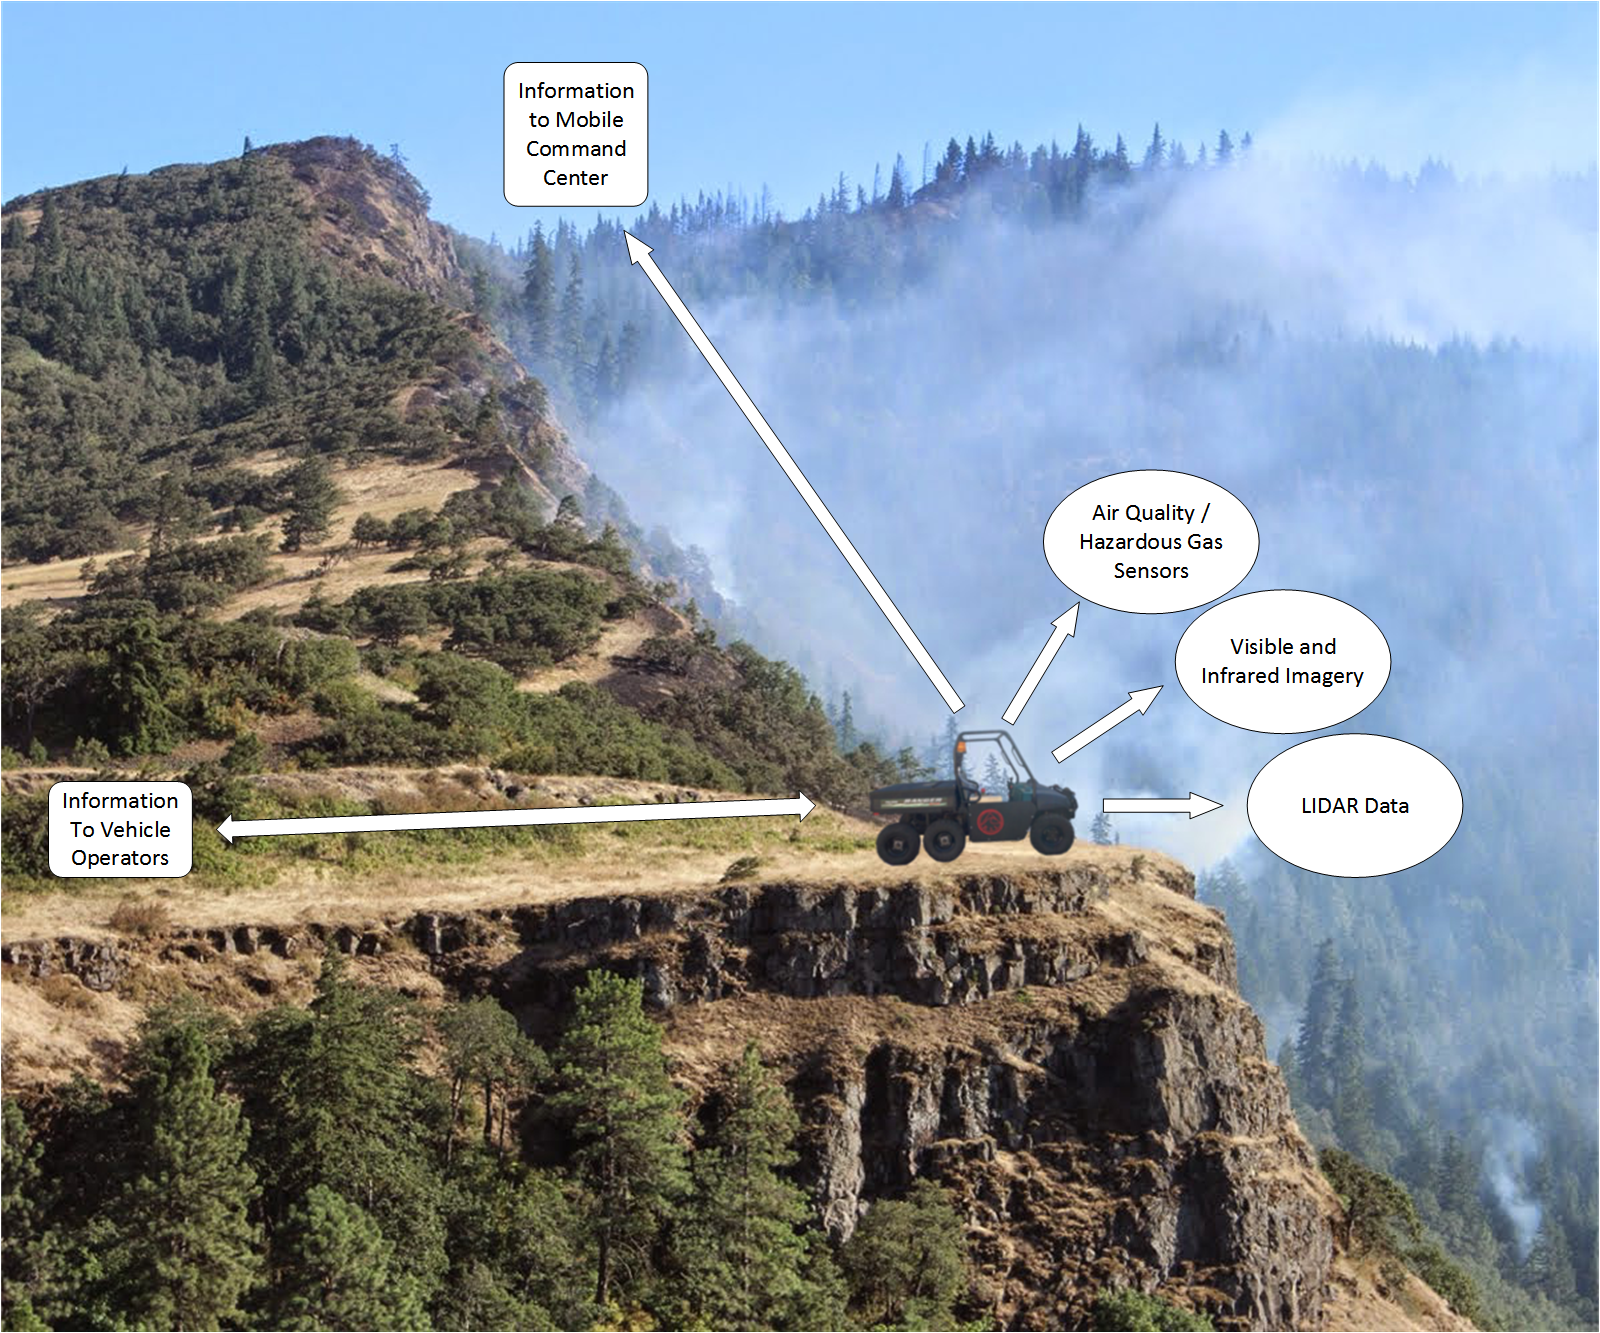
\includegraphics[width=0.75\linewidth]{UseCaseIllustration}
\caption{Use Case Scenario Illustration}
\label{fig:usecase}
\end{figure}
For example, while conducting fire fighting operations, the fire fighters make the decision to send the rover into an area which has been flagged as potentially hazardous. The operators manually operate the vehicle to position themselves and their gear near the danger zone. The operators can then quickly dismount and setup the teleoperation command center. The vehicle then proceeds into the potentially toxic environment, measuring the concentrations of potentially toxic, airborne substances and relaying that information back to the operators. While one operator focuses on driving the vehicle, an analyst focuses on the sensor streams, including the environmental sensors, monitoring harmful gas concentrations, and the LIDAR data, identifying physical obstacles which may be difficult to see in a visually impaired environment. Both operators will also relay, via a satellite communications link, images, videos and data to the forest fire fighting mobile operations center where strategists can best decide how to proceed with fire fighting operations. (See Fig \ref{fig:usecase})
%--------------------------------------------------------------------------------
%
%--------------------------------------------------------------------------------
\section{Functional Analysis}
% Functional decomposition (main functions and subfunctions)
% Specific lists of inputs/ outputs, constraints (summarize here, details in appendix)
%Block Diagrams
\begin{figure}[H]
\centering
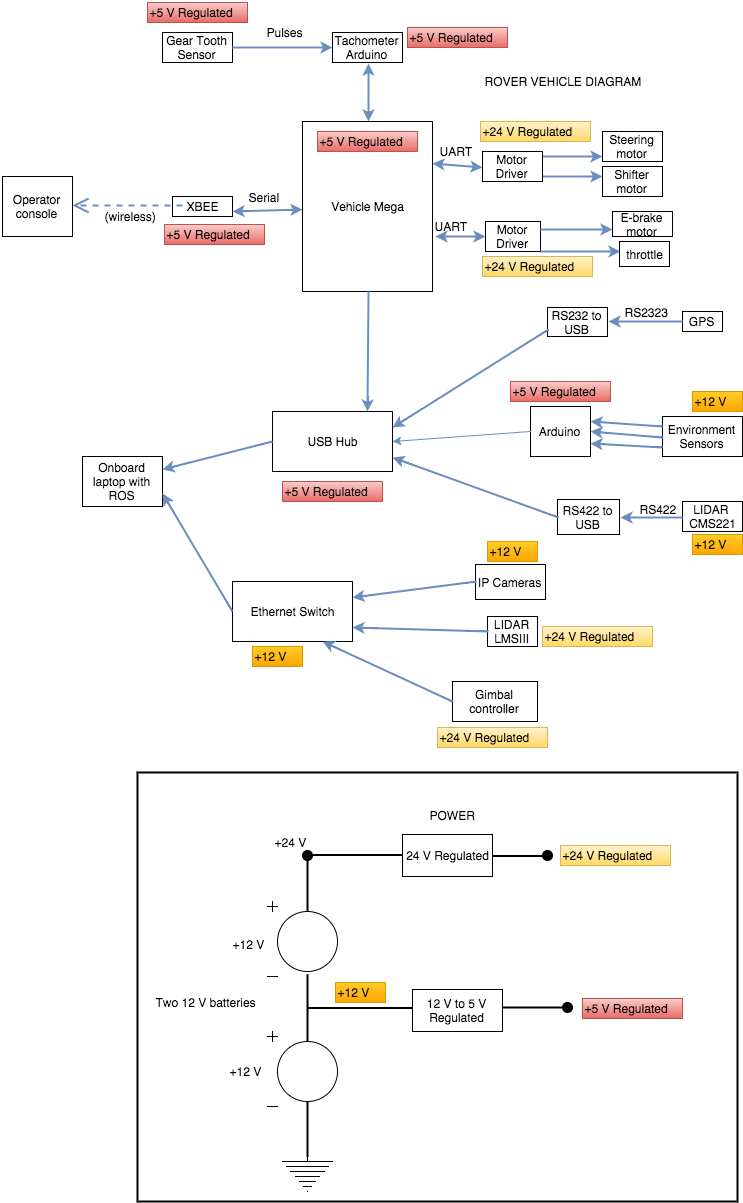
\includegraphics[scale=0.5]{Mech-elen_Component_Block_Diagram}
\caption{Mech/Elen Component Block Diagram}
\label{fig:mechelencomponentdiagram}
\end{figure}


\begin{figure}[H]
\centering
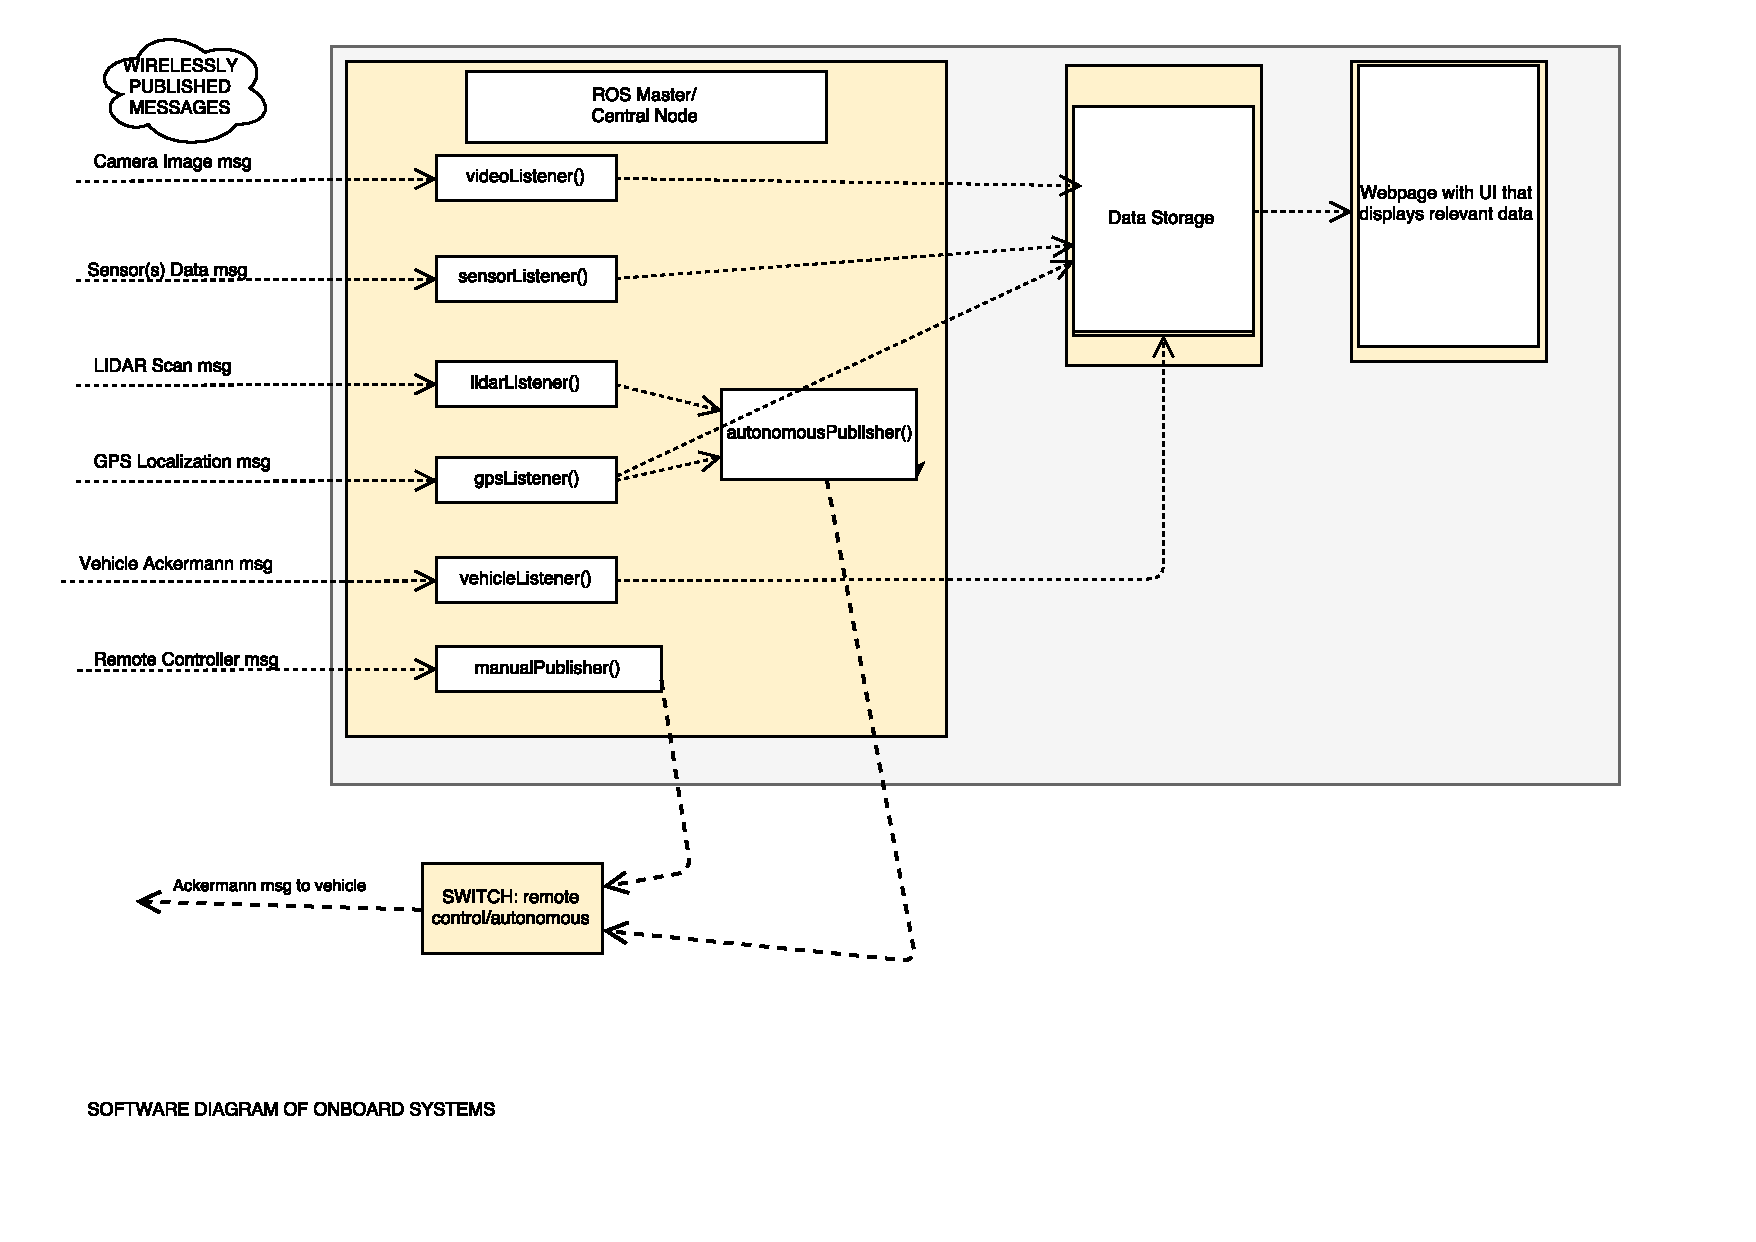
\includegraphics[scale=0.45]{Software_Component_Diagram}
\caption{Software Component Block Diagram}
\label{fig:softwarecomponentdiagram}
\end{figure}


%Subsystems
The vehicle is categorized into five subsystems: environment sensing, operator control and user interface, communications, power, and localization. The breakdown of the two primary systems, hardware and software, can be seen in figures \ref{fig:mechelencomponentdiagram} and \ref{fig:softwarecomponentdiagram} and show how these subsystems fit together. The environment sensing subsystem includes the sensor packages, cameras, and LIDAR units. The operator control and user interface subsystems are the systems that control the vehicle remotely as well as the data presentation components. The vehicle must communicate back and forth with the operator, receiving driving commands and sending data readouts. This is categorized under the communications subsystem. All powering is classified by the power subsystem. The final subsystem is labeled localization and it includes the ROS architecture involved with determining vehicle position for accurate mapping. \\
%--------------------------------------------------------------------------------
%
%--------------------------------------------------------------------------------
\section{Benchmarking Results}
% Whats out there that's similar
Many all-terrain, unmanned vehicles on the market are for military contracts exclusively. However, Northrop Grumman and Argo Robotics both have products that fit the category of an unmanned, all-terrain vehicle that can be equipped with sensor packages for non-military purposes. Some of the specs for these products can be found in Table 2.1. These are the Argo J5 Mobility Platform (Fig \ref{fig:ArgoPlatform1}) at thirty-nine-thousand dollars, the Northrop Grumman Andros F6 (Fig \ref{fig:NorthropAndros1}), and the Northrop Grumman Wheelbarrow Mk9 (Fig \ref{fig:NorthropWheelbarrow1}). Prices for the two later vehicles are not available without a direct quote. 

\begin{table}[H]
\begin{adjustwidth}{-.5in}{-.5in}
\centering
\begin{tabular}{c|c|c|c|c|c}
Product & Height(m) & Width(m) & Length(m) & Sensor Packages & Features\\\hline
J5 Mobility Platform & 0.83 & 1.38 & 1.52 & 1 Camera Mount & Amphibious\\
Andros F6 & 1.486 & 0.445 & 1.32 & 5 Cameras & Extendable Arm \\
Wheelbarrow Mk9 & 1.24 & 0.63 & 1.24 & Up to 10 Cameras & Extendable Arm\\
\end{tabular}
\caption{\label{tab:current} Current Product Comparison}
\end{adjustwidth}
\end{table}

\begin{figure}[H]
\centering
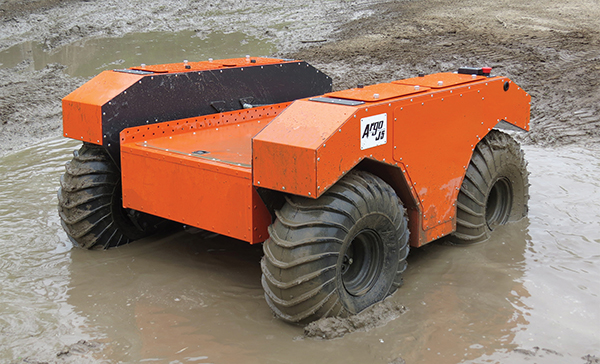
\includegraphics[width=0.5\textwidth]{argo-j5-mobility-platform-2-small-1.jpg}
\caption{Argo J5 Mobility Platform}
\label{fig:ArgoPlatform1}
\end{figure}


\begin{figure}[H]
\centering
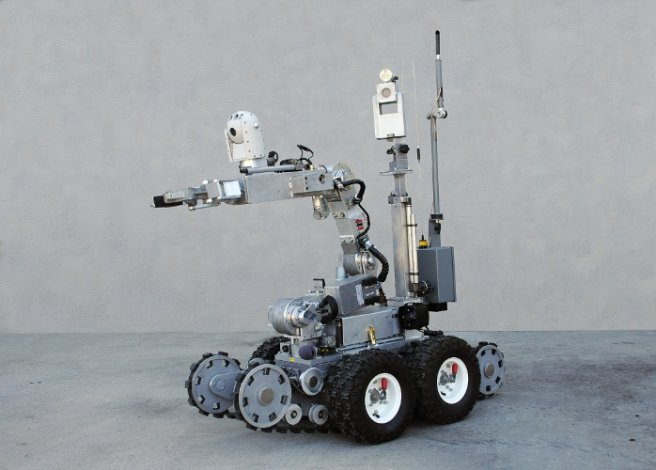
\includegraphics[width=0.5\textwidth]{NG1.jpg}
\caption{Northrop Grumman's Andros F6}
\label{fig:NorthropAndros1}
\end{figure}

\begin{figure}[H]
\centering
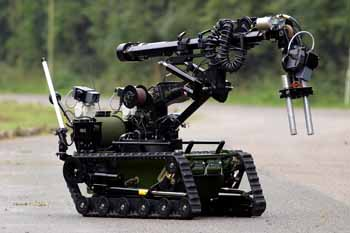
\includegraphics[width=0.5\textwidth]{wheelbarrow.jpg}
\caption{Northrop Grumman's Remotec Wheelbarrow Mk9}
\label{fig:NorthropWheelbarrow1}
\end{figure}

While these products that are on the market are the most similar to the product we wish to produce, the issues we wish to address are not solved by these rovers. Both of Northrop Grumman's rovers do not have the housing needed for sensor packages necessary to respond to forest fires. The Argo rover also does not house the necessary data packages, and while it is amphibious, it has been decided that sensor housing is more important.

Other Aerial Drones are also in the market for unmanned vehicles capable of relaying data such as thermal imaging and video back to the user. Two such products are the Elimco UAV-E300 (Fig \ref{fig:ElimcoUAVE3001}) and the Sensefly's EBee (Fig \ref{fig:SenseflyEBee1}). Both of these products have the capabilities necessary to map and relay usable data, and are marketed as disaster response vehicles. However, there are some inherent weaknesses to their aerial nature. Mr. Untamed has pointed out that images provided by Aerial vehicles can oftentimes be unusable as smoke can sit on top of the canopy of a forest, especially in the mornings. They also can only provide overhead data, and may not be able to map certain elements disaster responders could need, such as air quality at ground level or mapping paths that are safe. Our vehicle seeks to get under this layer of smoke to provide data from the ground level.

\begin{figure}[H]
\centering
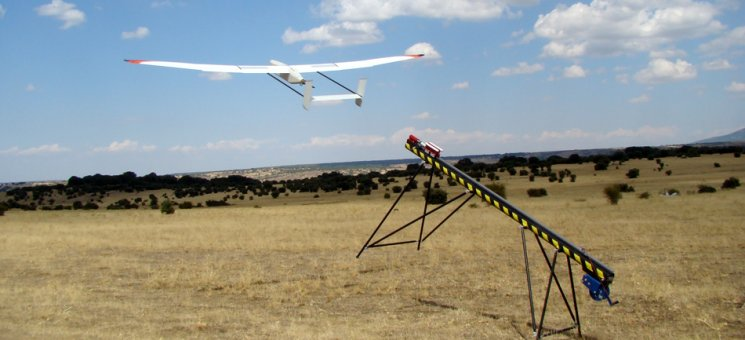
\includegraphics[width=0.5\textwidth]{UAV-E300.jpg}
\caption{Elimco UAV-E300}
\label{fig:ElimcoUAVE3001}
\end{figure}

\begin{figure}[H]
\centering
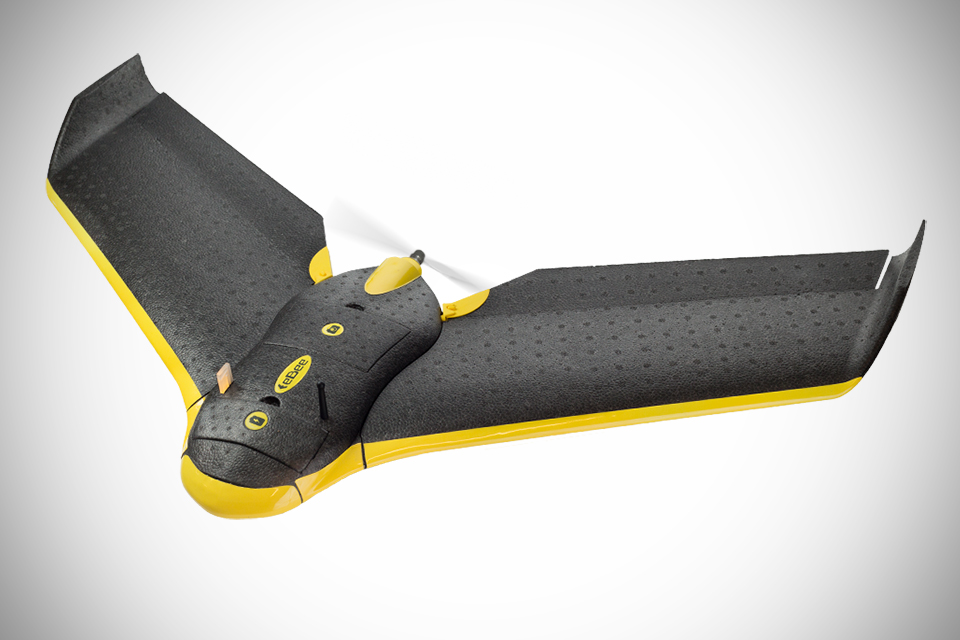
\includegraphics[width=0.5\textwidth]{e-bee.jpg}
\caption{Sensefly's UAV EBee}
\label{fig:SenseflyEBee1}
\end{figure}
%--------------------------------------------------------------------------------
%
%--------------------------------------------------------------------------------
\section{System Level Issues, Trade-off Analysis}
The design process for this vehicle required that we opt for certain configurations and components over alternatives. The biggest design decisions we had to make were on the LIDAR layout and environmental sensing systems.\\

\subsection{LIDAR Physical Configuration}

Two LIDAR units, a SICK LMS221 on a pivoting mount (Fig \ref{fig:lms221A}) capable of generating a 3D point cloud and SICK LMS111 2D linescan LIDAR (Fig \ref{fig:lms111A}) capable of producing 2D obstacle maps, were made available to our team through Santa Clara's  Robotic Systems Lab. One design challenge was to determine the optimal location for these two sensors on the vehicle. The total combined field of view, blind-spots, total weight, material cost, view height and vehicle vertical clearance were all taken into account when deciding on the configuration. 

\begin{figure}[H]
\centering
\begin{subfigure}{.5\textwidth}
  \centering
  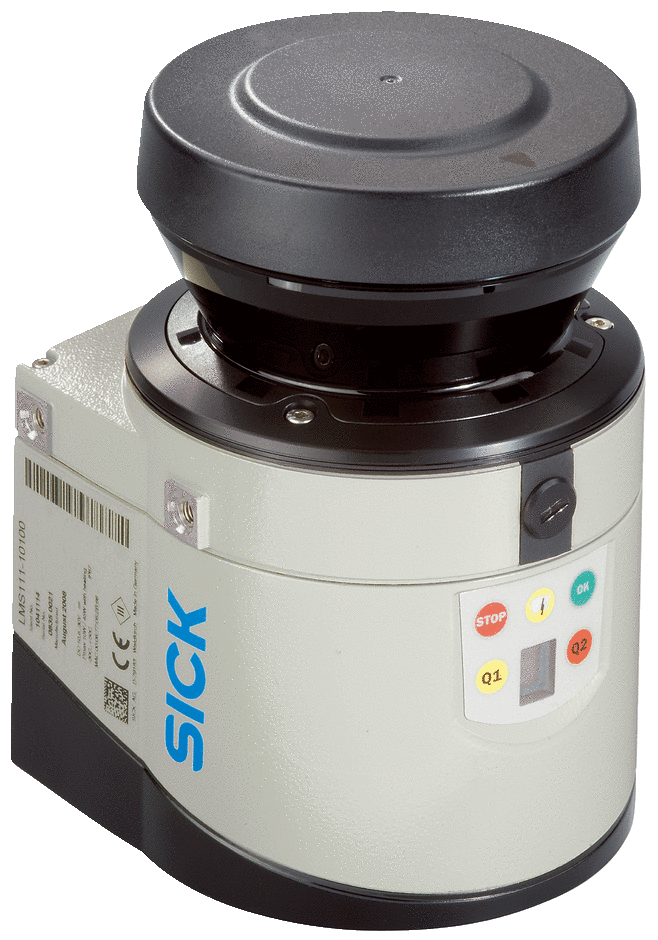
\includegraphics[height=.5\linewidth]{LMS111}
  \caption{LMS 111: 2D LIDAR}
  \label{fig:lms111A}
\end{subfigure}%
\begin{subfigure}{.5\textwidth}
  \centering
  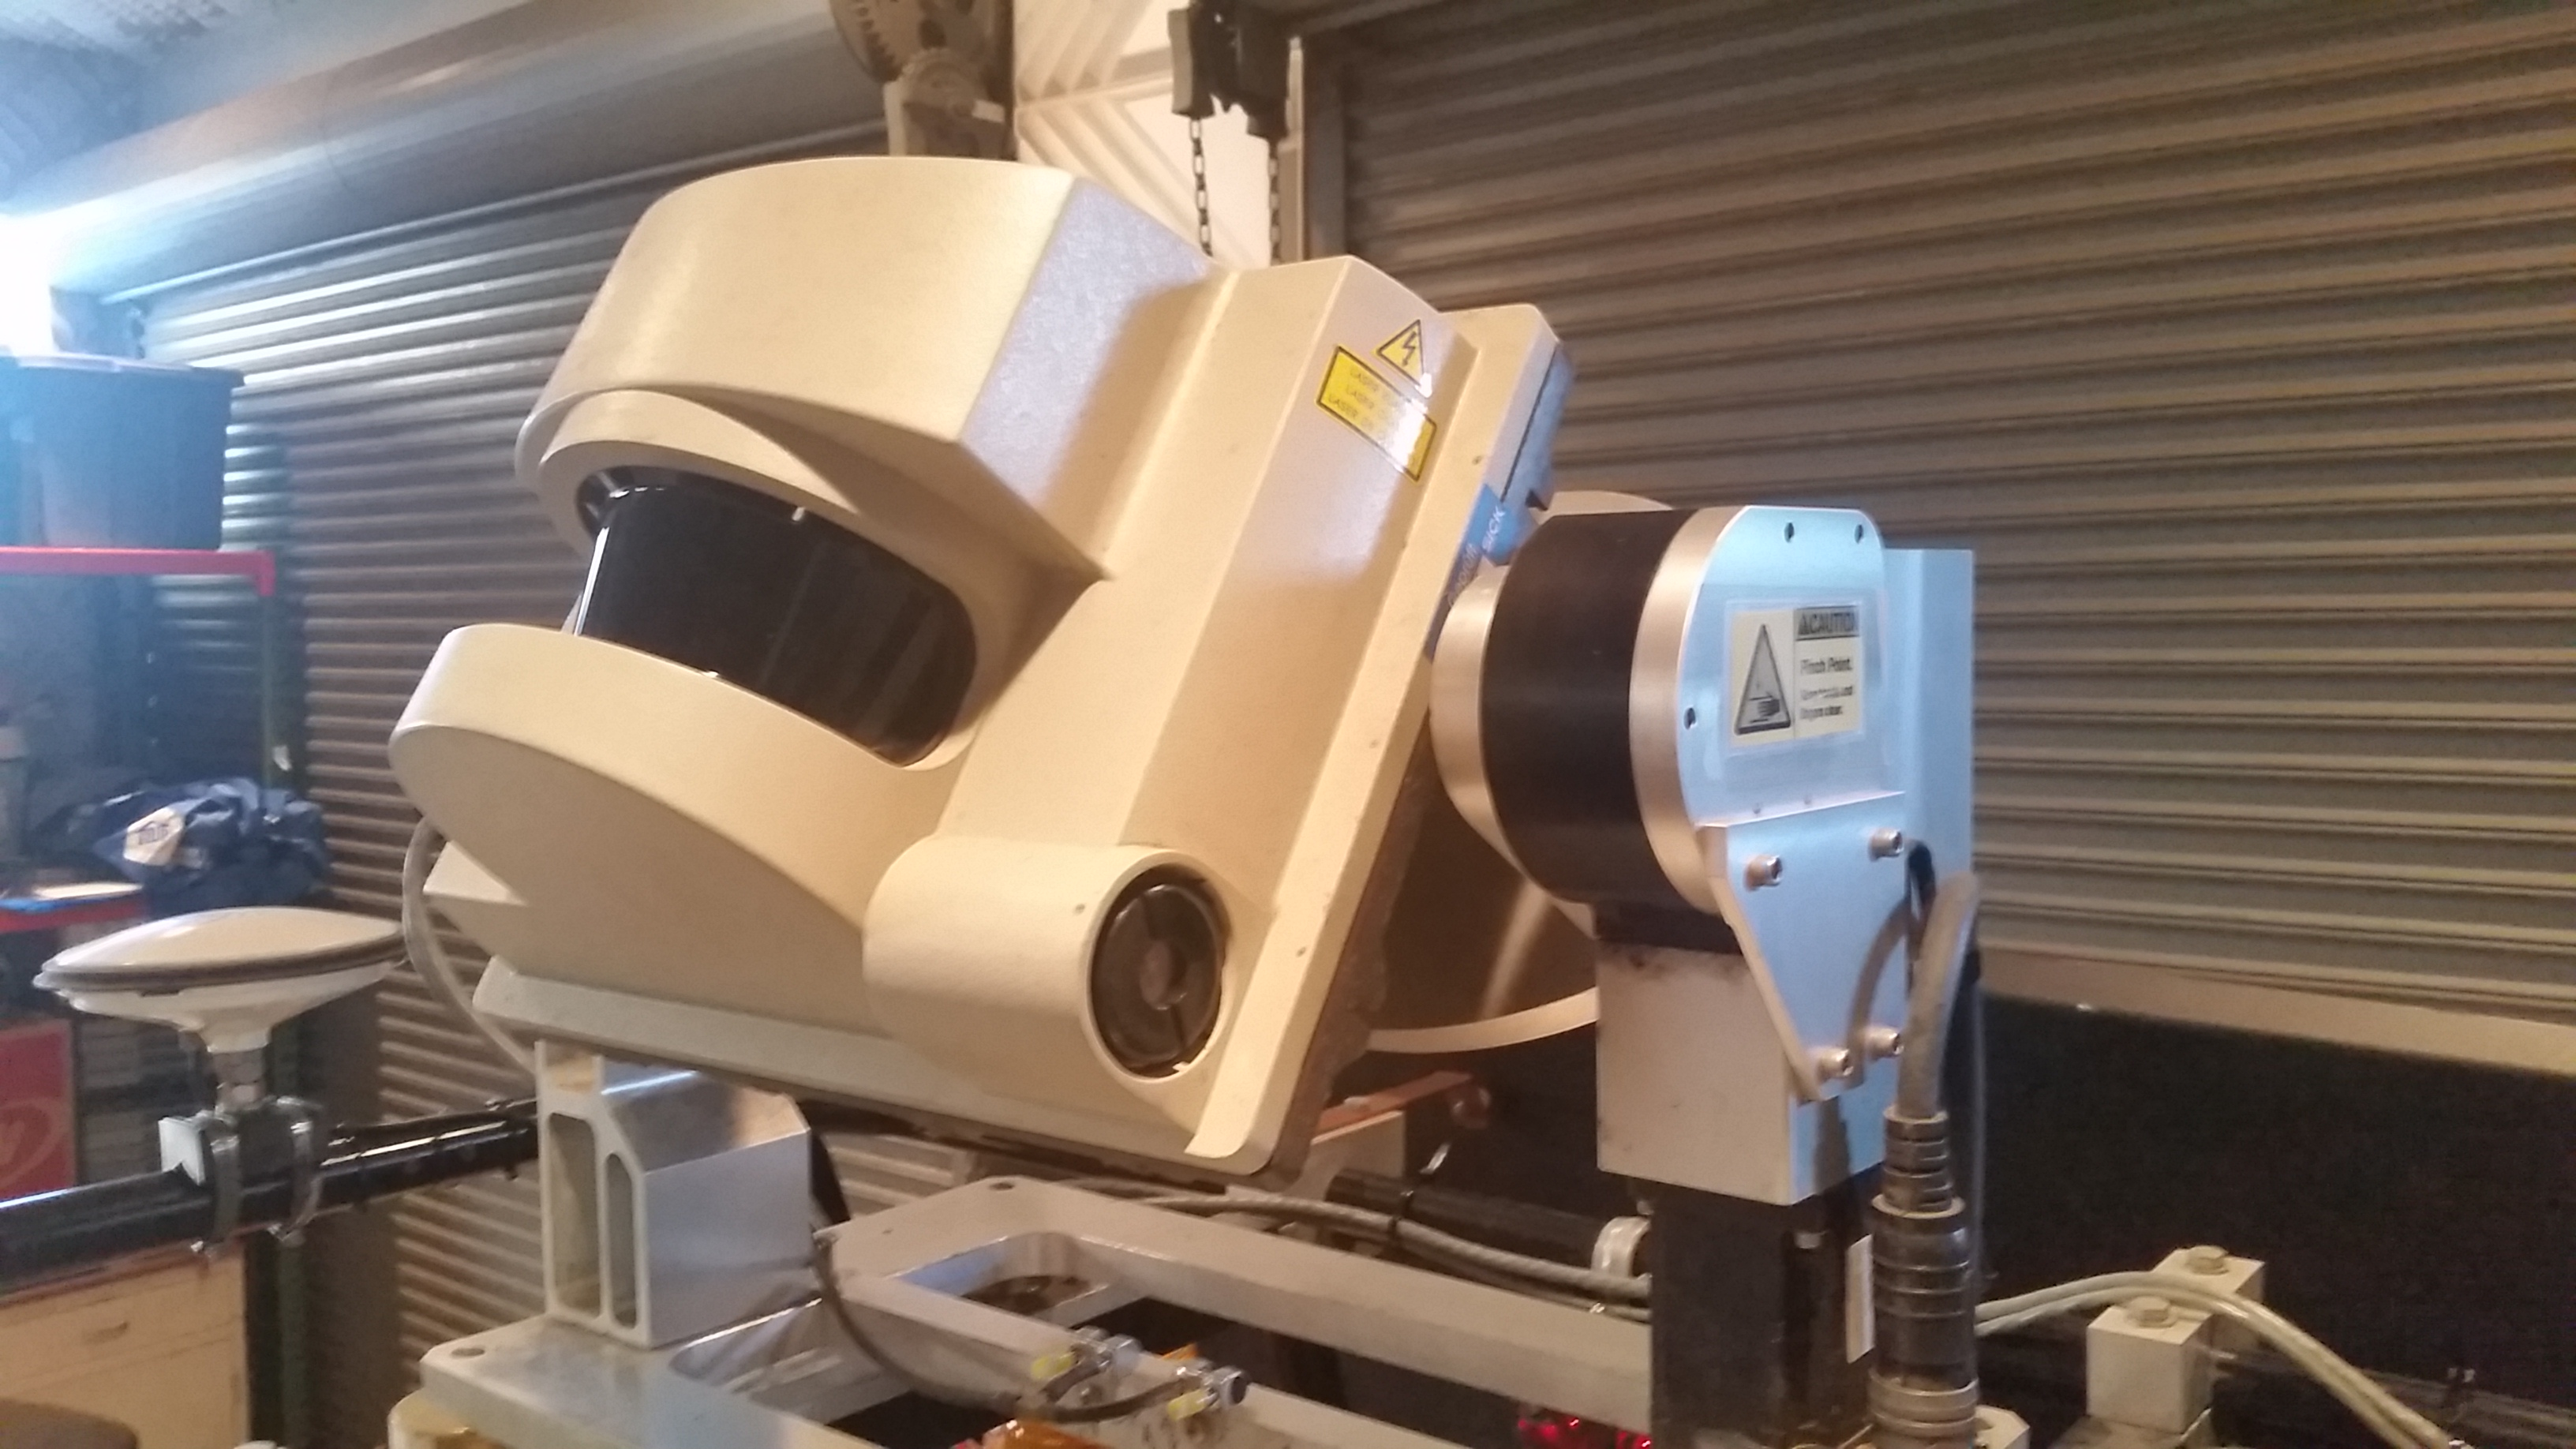
\includegraphics[height=.5\linewidth]{LMS221}
  \caption{LMS 221: 3D LIDAR}
  \label{fig:lms221A}
\end{subfigure}
\caption{LIDAR Types}
%\label{fig:ddd}
\end{figure}

A final configuration was chosen based on the Concept Scoring Tradeoff Analysis in Appendix \ref{App:tradeoff}. The final configuration has the 3D, articulated LIDAR (LMS221) mounted on the top of the roll cage where it has a full forward and rear field of view. The 2D LIDAR (LMS 111) has been mounted on the front grill of the vehicle where it can mitigate a blind spot immediately in front of the vehicle. 

%TODO: PICTURE OF FINAL CONFIGURATION SKETCH

\subsection{Sensor Physical Configuration}
%Environment sensing
%Add/change what sensors we will have in paragraph below
The hazardous environment sensing requirement has been filled by three redundant sensor packages placed on the hood and each side of the roll cage (See Figure \ref{fig:systemlayout}). The sensor packages  are enclosed in a box with a forced air inlet to continually monitor the air for changes in composition while also protecting the components. The enclosed array of sensors are able to detect temperature and concentrations of: carbon monoxide, methane, carbon dioxide, hydrogen, air particulate, and liquefied petroleum gas. The cost of an oxygen sensor is prohibitive, so oxygen concentrations must be extrapolated from alternative sensors. These sensors could be expanded as needs arise. The vehicle is equipped with redundant packages for a multitude of reasons. If a sensor fails, there are two other identical sensors to fill that role. Additionally, having the sensors spread out on the vehicle, it can be determined if concentration readings are representative of the greater area, certain elevations, or a single point. The data from the redundant sensors could be analyzed in three ways; the greatest reading could be displayed, the reading most common among sensors, or all three could be displayed. The first option, outputting the highest value, is the most conservative option while also being concise, but it makes it possible that false data could be transmitted. The most thorough method would be to transmit all three data streams and allow the operator to decide which to trust. 

The location of the air quality sensors and cameras was the next critical design decision. For the cameras, the field of view, mounting costs, implementation time and robustness, among other factors, were considered when deciding on a final design. Additionally, for the environmental sensors, the cost, implementation time, robustness and proximity to the vehicle's exhaust systems were considered when deciding on a sensor configuration. Appendix \ref{App:tradeoff} features a complete tradeoff analysis for the sensor configurations. 

\begin{figure}[H]
\centering
\begin{subfigure}{.5\textwidth}
  \centering
  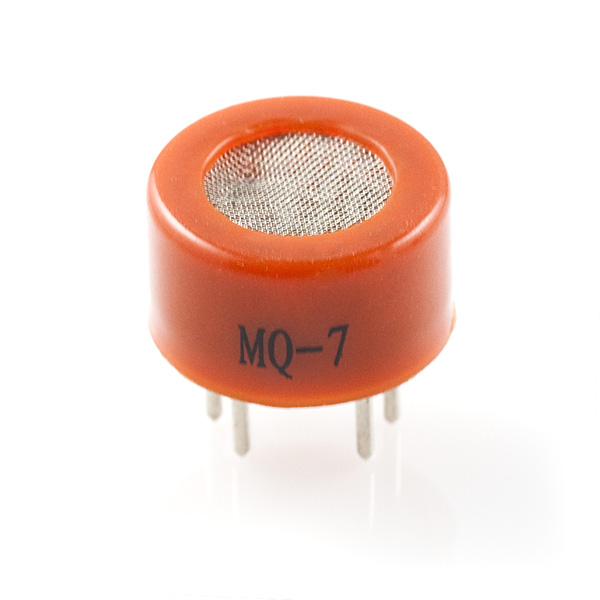
\includegraphics[height=.5\linewidth]{cosensor}
  \caption{Carbon Monoxide Sensor}
  \label{fig:sub1}
\end{subfigure}%
\begin{subfigure}{.5\textwidth}
  \centering
  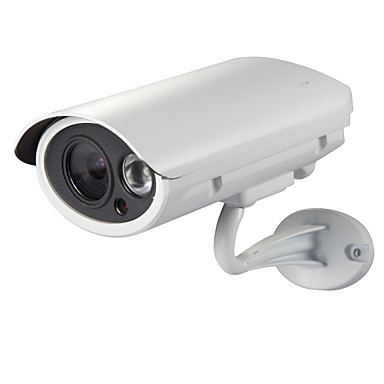
\includegraphics[height=.5\linewidth]{camera}
  \caption{IP Camera}
  \label{fig:sub2}
\end{subfigure}
\caption{Sample Sensor Types}
\label{fig:sensortest}
\end{figure}

A final configuration was chosen where the cameras are mounted on all 4 sides of the roll cage, allowing full coverage of the surroundings while also allowing the operator to see over obstacles. The redundant sensor packages are  located on the front of the roll cage and on the front of the vehicle. 

 
%--------------------------------------------------------------------------------
%
%--------------------------------------------------------------------------------
\section{System Level Architecture}
% Layout of system-level design with main subsystems

\begin{figure}[H]
\centering
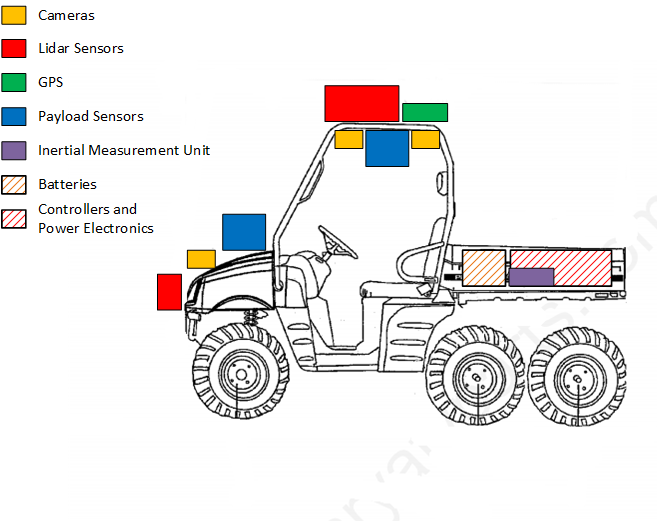
\includegraphics[width=.7\linewidth]{SensorLayout}
\caption{System Layout Architecture}
\label{fig:systemlayout}
\end{figure}
%--------------------------------------------------------------------------------
%
%--------------------------------------------------------------------------------
\section{Team and Project Management}

As the RSL Rover project is a continuing project through Santa Clara's Robotic System's Lab, we were provided with a workshop right off of the engineering quad which is outfitted with computers, tools and workspaces. We were also provided some financial assistance in purchasing some tools which will stay with the RSL and will continue to be used by teams in the future. 

One of our major constraints is our budget. We were awarded a grant of \$2500 from Santa Clara's School of Engineering (Undergraduate Programs Funding). We used this funding to purchase sensors and raw materials for the environmental sensing packages, repair the vehicle and purchase various electronic components in order to support the new computing and sensing packages. A complete, line-item budget can be found in Appendix: \ref{App:Budget}. 

Due to the scope of our project, an accelerated timeline was required. During fall quarter, we successfully integrated GPS and LIDAR sensors, including power and communication systems, onto the vehicle and successfully integrated these sensors, along with driving functionality to the ROS (Robot Operating System) software platform. During winter quarter we designed the environmental sensing packages, and integrated cameras and an inertial measurement unit on the vehicle and began development on a web-based GUI application to present this data to first responders. During spring quarter we successfully integrated all of our subsystems and ran extensive field testing to validate our design against our engineering requirements. See Appendix \ref{App:Gantt} for a complete Gantt chart summarizing our schedule. 

We as a team have dedicated ourselves to this task, in the hopes of completing the listed goals by the end of the year. We held each other accountable by meeting at least twice a week, once under the supervision of our advisor and once on our own. At each meeting, we went over the work we had done in the previous week and talked about tasks, and who would be best suited to handle each task. Patrick Barone has served as the primary leader of the group, however, each of us has taken initiative in leading the group on different occasions or when undergoing certain tasks. Despite the fact that we are split between two majors, we have been able to always communicate effectively about our projects, successes, failures, and insights to others. We have all contributed to the project as a whole and to the research process in order to inform our design. 

To begin our design process, we first assessed the state of the vehicle as it had already been modified by two Senior Design teams in previous years. From there, we assessed how the rover could be changed, fixed, or left as is in order to make it best suited for disaster response, especially in the case of forest fires. During this time, we researched what was actually needed in these disasters by interviewing disaster responders and reviewing literature; in addition, we researched current solutions and similar market products, paying close attention to their strengths and shortcomings. We then created a criteria for ourselves and set goals and a timeline. We then began to design our system layouts, while assessing each possible design choice to find the best choice. 

This project, as a full sized, unmanned vehicle that will enter disaster sites, is subject to many risks, but we have sought to manage these risks as we feel this project is worth undertaking. First, as this project is unmanned, we run the risk of working with technology that the public has not yet fully accepted. Many see robotic technology as something to fear. In order to address this fear, we designed our system as a whole to make our vehicle not only functional, but also  intuitive and aesthetically pleasing.

Also, as an unmanned vehicle, there is no human to make snap decisions, such as braking. In order to mitigate these risks, we have leveraged the already-existing emergency stop button system that can quickly and effectively stop the vehicle from the human controlling the system, or viewing the data the rover is outputting. This will allow human controllers of the rover to have the power to make the snap decision to stop the device before anything bad can happen. For example, during our testing if we observe that the vehicle is not driving as anticipated and it is on course to hit an object (or even a person) we can quickly stop the vehicle.

As the vehicle is fully-sized, our team ran the risk of causing injury to ourselves and others as we put the car up on jacks to work with it; consequently, we have established safety guidelines in order to ensure that we kept ourselves and guests working on the machinery with us safe. The approved safety protocol is included in \ref{app:safety}. As the vehicle itself is also a few years old, we ran the risk of it breaking down on us. To prevent this, the team has done extensive work, through preventative maintenance, to ensure that the rover is kept in a well maintained state. As for the risk of us putting the rover into unstable disaster sites, we ran the risk of the environment harming our equipment. We have conducted research on heat shielding in order to protect key features on our rover, however the solutions discovered were both cost prohibitive and also not critical to the robotic and sensing functionality that we aimed to prove through this project. That being said, we have also housed most of the delicate electronic equipment under a layer of protection. The roll cage, the hood, and the trunk cover all provide a sufficient level of protection for sensitive equipment. 


%% TODO: Gantt Chart
%% TODO: Budget Appendix